In this Chapter we will present the results of implemented the previously specified requirements that originated the Socii tool. As we previously mentioned we
choose a set of requirements (among a big list of possibilities) that would allows us to have a tool with the most relevant and core functionalities
in order to prove our hypothesis of building a web based \glspl{sna} tool.\\
\indent Along the Chapter we will not only list results but show them as well, in some of the following sections we present a set of Socii images that depict the implemented functionalities and how to use them. In a more final part of this Chapter we present a case study, were we analyze a real network and derive some different conclusions that well demonstrate some of the use cases of Socii.

\section{Note about the final results}

As the development of the tool depended on the \glspl{osn} integration and real data analysis, we had to somehow manage to fed real data sets into
Socii. The way we achieve this was not an totally automatic process, we used the crawler modules and extraction \glspl{api} mentioned and very well explained in Chapter 5 and 6, to extract real data sets into a local filesystem, and then with a migration script we pointed to the production MongoDB instance in order to store the real data so that Socii aggregator component could get the real data. To improve data feeding interoperability we have two functionalities working side by side, the user may choose to analyze a real network (previously extracted by the mentined process) or the user may choose to generate a network with data from our generators module.


\section{Final Results Summarization}

The following table summarizes the features that were implemented on Socii. All the "\textbf{MUST}" requirements were implemented
and two additional "\textbf{SHOULD}" requirements were also implemented since they were almost cost free once we had the
component react-d3-graph in a more advanced stage. As mean of summarization we will present a table concisely points to
each requirement with the proper reference that we created in Chapter 6.

\begin{table}[H]
\renewcommand{\tabcolsep}{2pt}
\begin{tabular}{ |c|l|c| }
\hline
\textbf{Requirement} & \textbf{Short Description} & \textbf{Status}\\
\hline
6.3.2, 1 & Socci login & \ding{51}\\
\hline
6.3.2, 2 & Order network build (extraction simulation) & \ding{51}\\
\hline
6.3.2, 3 & Extraction feedback & \ding{51}\\
\hline
6.3.3, 1 & Render network & \ding{51}\\
\hline
6.3.3, 2 & Community detection (visually identifiable) & \ding{51}\\
\hline
6.3.3, 3 & Drag and Drop all network & \ding{51}\\
\hline
6.3.3, 4 & Zooming interactions & \ding{51}\\
\hline
6.3.3, 5 & Interactive node comparison & \ding{51}\\
\hline
6.3.3, 6 [\textbf{SHOULD}] & Global network interactions (Toolbar) & \ding{51}\\
\hline
6.3.3, 7 [\textbf{SHOULD}] & Disable heavy animations & \ding{51}\\
\hline
6.3.2, 1 & Network Generator (Facebook) & \ding{51}\\
\hline
6.3.2, 1 & Network Generator (LinkedIn) & \textbf{On Hold}\\
\hline
6.3.2, 2 & Network Generator - Configuration & \ding{51}\\
\hline
6.3.3, 4 & Zoom network & \ding{51}\\
\hline
6.3.3, 5 & Detect heavy network and disable animations & \ding{51}\\
\hline
6.3.4, 1 & Render label along side each node & \ding{51}\\
\hline
6.3.4, 2 & Highlight node and adjacent connections & \ding{51}\\
\hline
6.3.4, 3 & \begin{tabular}{@{}l@{}}Node click and show information\\ (network metrics and information in\\ the context of the \glspl{osn})\end{tabular} & \ding{51}\\
\hline
6.3.4, 4 & Drag and Drop nodes & \ding{51}\\
\hline
6.3.5, 1 & Render network links with \textit{semantic thickness} & \ding{51}\\
\hline
6.3.8, 1 & Download network in the format GraphML & \ding{51}\\
\hline
6.3.9, Facebook, 1 & Sentiment Analysis & \textbf{In Progress}\\
\hline
\end{tabular}
\caption{\label{table:featuresocii} Summarization of Socii features.}
\end{table}

In the Table \ref{table:featuresocii} we present a list of the implemented requirements, these refer to the requirements in Chapter 6. All the requirements are \textbf{MUST} requirements unless otherwise is stated.

\section{Socii - final aspect and functionalities overview}
In this section we do an overview across Socci application, we present the overall functionalities that Socii offers
from an end user perspective.

\subsection{Network Configuration Area}

\subsubsection*{Entry state}

\begin{figure}[h!]
\begin{center}
  \hspace*{-0.8in}
  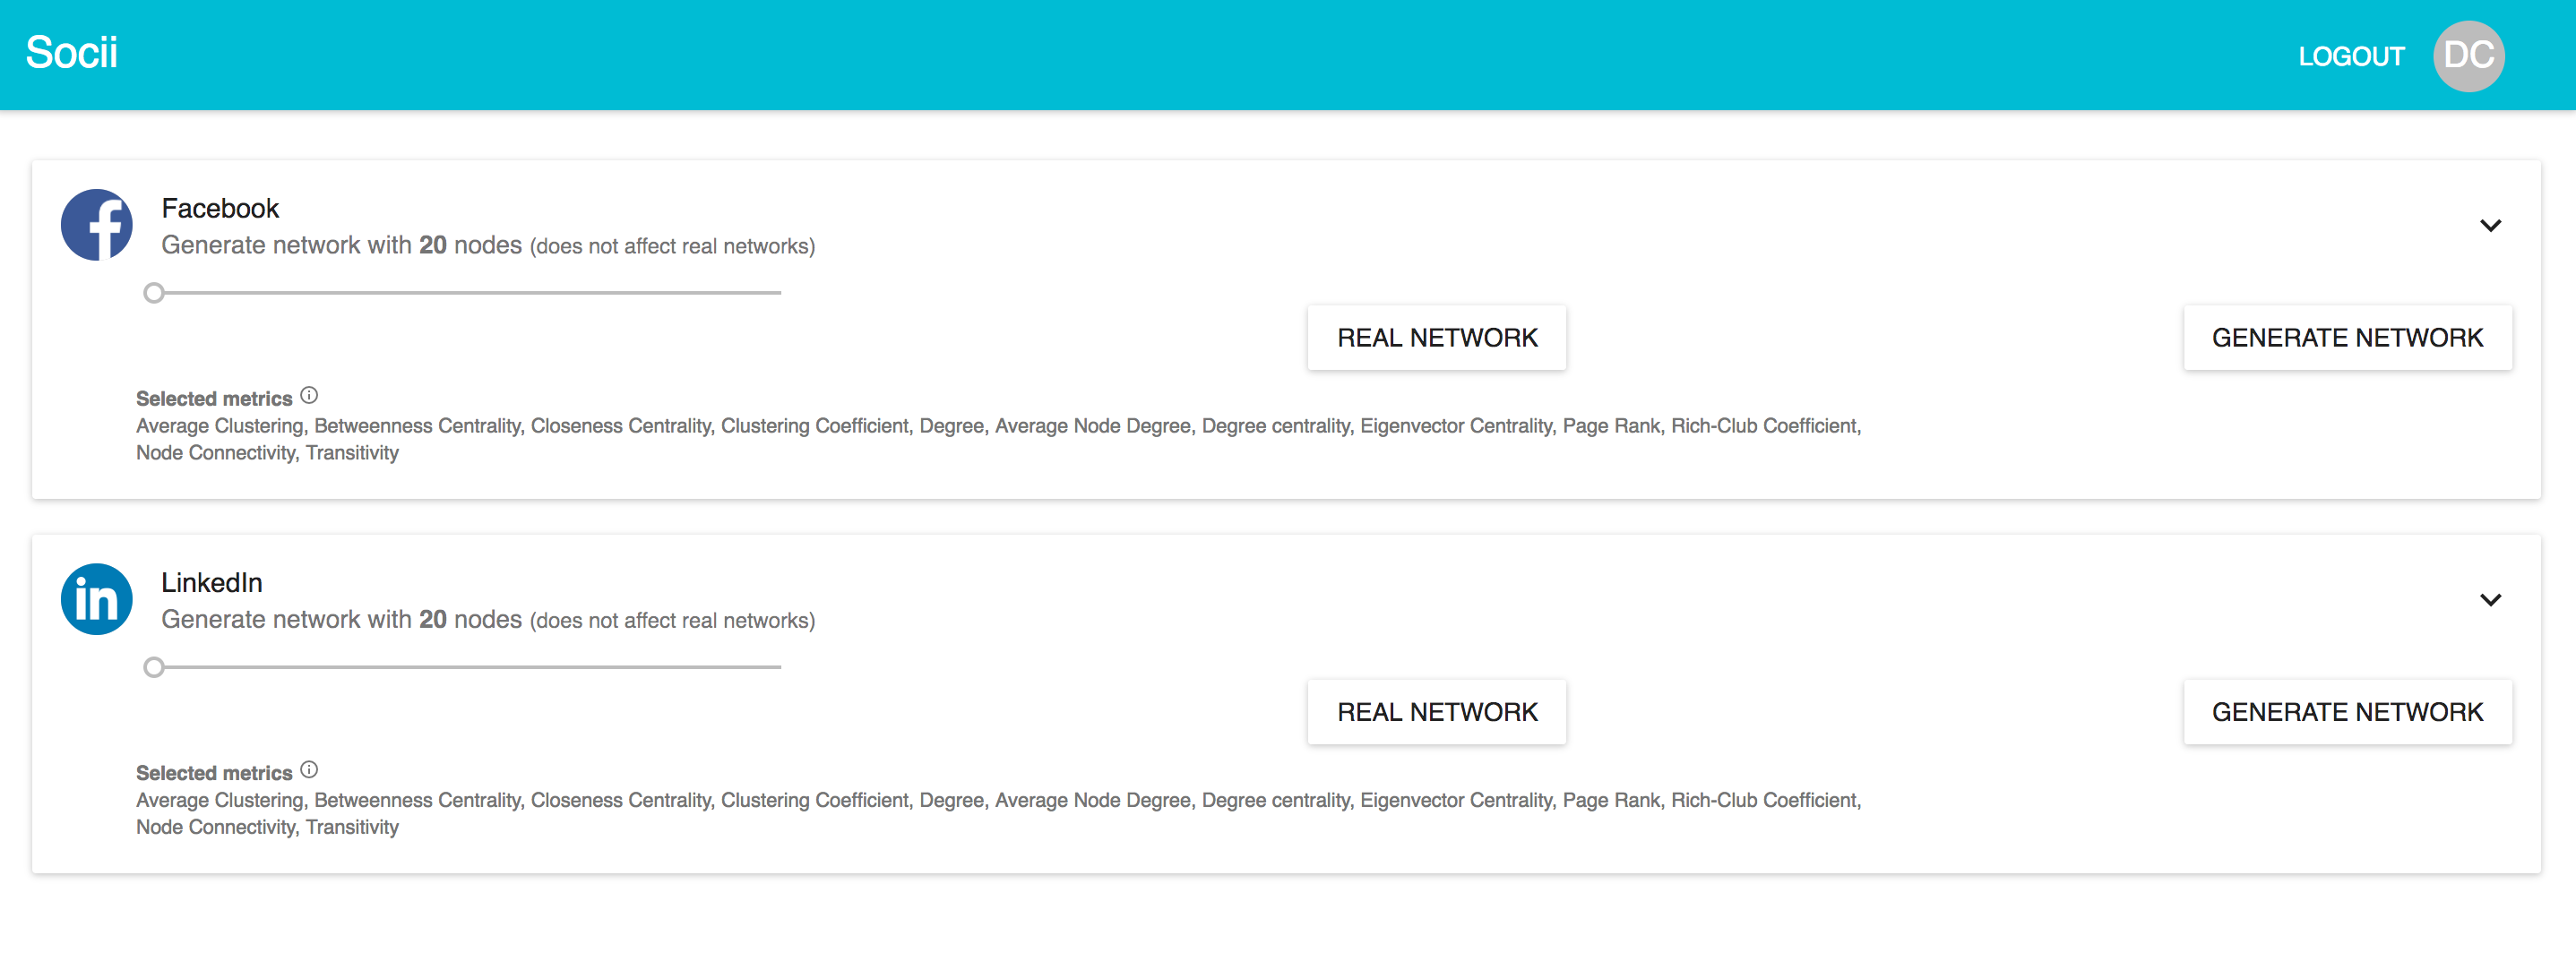
\includegraphics[width=1.2\textwidth]{img/socii/socii_1.png}
\end{center}
\caption{\label{img:socii_1} Socii landing page. Network configuration area.}
\end{figure}

In Figure \ref{img:socii_1} we may observe our initial page where we display available \glspl{osn} that can be configured in this area and then a network generation or network calculation upon real network may be ordered. Each \glspl{osn} consists in a expandable card that once expanded contains all the details and information about the \glspl{osn} and metrics configuration.

\subsubsection*{Configuration card detail}

\begin{figure}[h!]
\begin{center}
  \hspace*{-0.8in}
  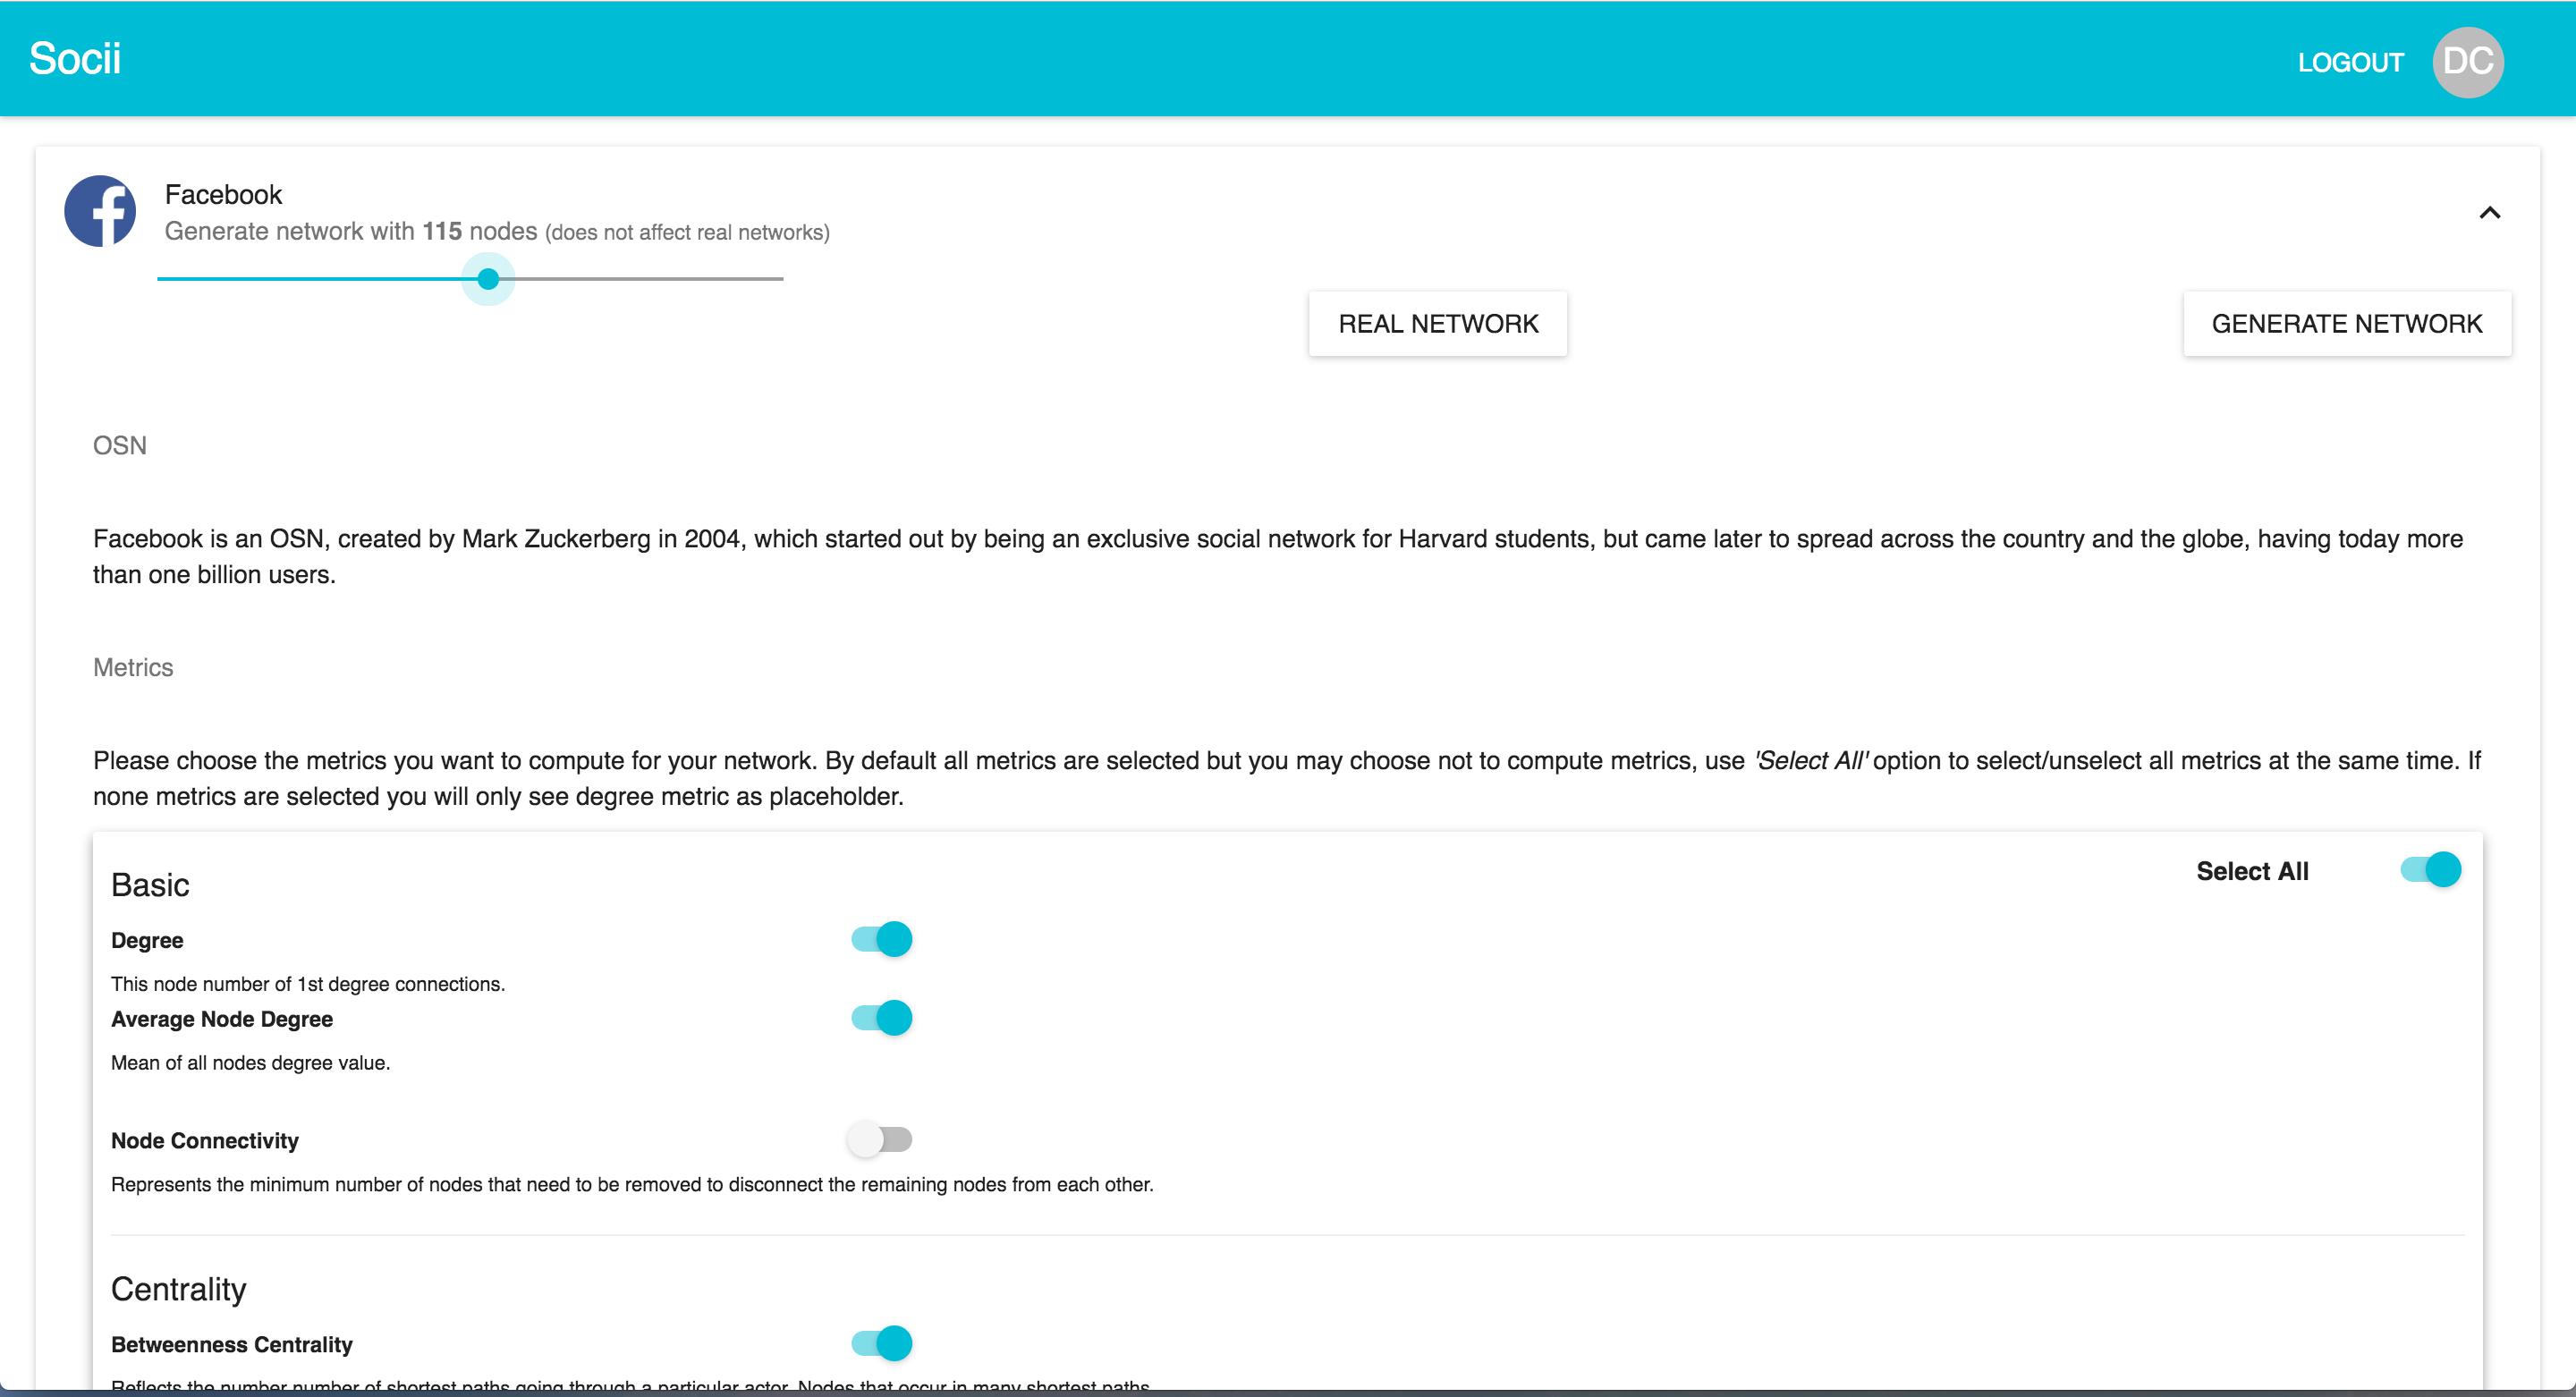
\includegraphics[width=1.2\textwidth]{img/socii/socii_2.png}
\end{center}
\caption{\label{img:socii_2} Network configuration area. Facebook configuration expanded.}
\end{figure}

In Figure \ref{img:socii_2} Facebook configuration card is expanded and here we see that we can have a great level of granularity upon the \glspl{sna} metrics that we want to calculate against a certain network. On the top of the card we have a brief description of the \gls{osn} followed by sections that represents sets of metrics, and for each one of the metrics we also provide a brief explanation for a given metric.\\
\indent These are the metrics that we will then be able to see for each node in the network visualization area. To reach more flexibility we decide on switches visual elements to turn on/off a certain metric, by doing this we may combine any set or subset of metrics. Some of the metrics are global (these mean that they are calculated regarding the graph/network in general) other are node specific (have a meaning at node level), this is implicit within each metric description.

\subsection{Network Visualization Area}
[TODO]

\subsubsection{Toolbar}
[TODO]

\subsubsection{Node Discovery}
[TODO]

\subsubsection{Node Details}
[TODO]

\subsubsection{Node Comparison}
[TODO]

\subsubsection{Community Detection}
[TODO]

\section{Case Study}
(...)
As we mentioned Socii uses generators to build a network for a given \gls{osn} with a specific required number of nodes. In this section we present
a real case study with real data in order to prove the accuracy of conclusions that Socii provides in a real context. For this case study we will use
a real account and extract information from Facebook using the facebook web crawler module that was developed initially as a back-end requirements to allow extraction on the fly, but not that being possible by the mentioned reasons, we use it as mean to obtain a real data set that we inject in Socii and associate to a whitelisted Socii account that besides being able of generating \glspl{osn} networks as normal users, the whitelisted users will also have available an option to consult a predefined network that is built on the fly with already stored data (the case study data).
(...)

\subsection{Socii Applications}

%% \subsubsection{Migration Flows} Painting nodes by city or country should have uniform colors and not redo coloring and stuff....
%% Use socii community detection to overlap.

\subsubsection{Marketing with community detection (Facebook)}
A real example within the case study. Study community preferences.

\subsubsection{Sentiment Analysis (Facebook)}
Society happiness studies/Depression detection.

\subsubsection{HR Discovery (LinkedIn)}
